\documentclass[11pt,letterpaper,]{article}
\usepackage[latin1]{inputenc}
\usepackage{amsmath}
\usepackage{amsfonts}
\usepackage{amssymb}
\usepackage{appendix} % Adds additional appendix support
\usepackage{graphicx} % Adds support for graphics
\usepackage{listings} % Adds support for syntax highlighting.
\usepackage{verbatim} % For shell output
\usepackage{fancyvrb} % Gives me some more options on verbatiminput
\usepackage{url} % For wikipedia
\usepackage{setspace}

\usepackage{float}


\author{Spenser Gilliland \& Richard Hanley}
\title{Project 3: Simulation of CPU Cache and \\ Memory Subsystem}

\begin{document}

\maketitle
\bigskip
\bigskip
\bigskip

\doublespacing

\begin{abstract}
%\paragraph{}
This report depicts the design process as well as simulation results of a memory hierarchy which includes a 512 byte instruction cache, 256 byte data cache and 2048 byte main memory.  The project was successful and the collected data is presented in section \ref{Results}.  This design is notable because the memory hierarchy was not only simulated but synthesized for an FPGA.  The results from synthesis are included in section \ref{Results:Synthesis}.  Furthermore, an assembler and linker were created to make it easier to experiment with different types of programs inorder to better assess the effectiveness of the memory hierarchy.
\end{abstract}

\pagebreak
\section{ Introduction }
\paragraph{}
This project presented an interesting opportunity to verify and evaluate the effectiveness of cache schemes on the performance of a computer program.  The programs that were evaluated were designed to find both worse case and best case performance as well as to show the effect of the locality of memory on the overall effectiveness of the processor. In addtion, the design and implementation of various memory hierarchy elements are shown.

\section{ Background }
\paragraph{}
In common processor based systems, it is highly likely that recently accessed data or instructions will be accessed again in the immediate future.  This is known as the data locality principle.  Memory hierarchies attempt to take advantage of expensive fast memories to hold this consistantly accessed data and slow cheap memories to hold the remaining data.  This results in a higher performance memory subsytem than raw access to the slow memory would normal entail.  This idea of including the commonly accessed instructions or data in a fast memory is called caching.

For the system at hand, there are a total of three memory elements arranged in the following memory hierarchy.

\begin{figure}[ht]
  \centering
  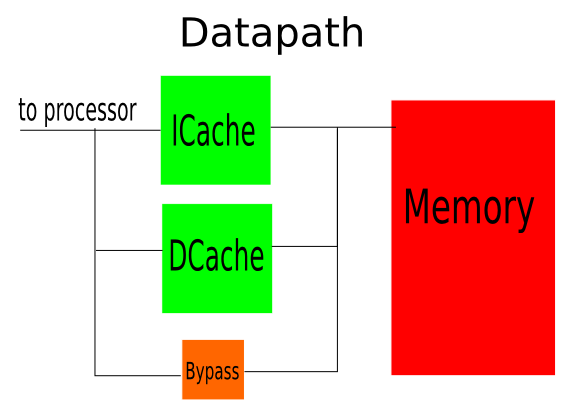
\includegraphics[width=4in]{img/datapath.png}
  \caption{ The datapath with Cache}
  \label{fig:datapath}
\end{figure}

\paragraph{Register File}
The register file is located inside the CPU.  It holds the registers that store the data immediately before ALU operations are performed on it.  The register file is the eventual location of all elements in memory and all of the data must go into the register file to be processed; therefore, this is almost always the fastest memory available, and is place in the die of the processor.

\paragraph{I-Cache \& D-Cache}
The I-Cache and D-Cache hold instructions and data, respectively.  These are expensive but fast memories which have single cycle access.  They transparently provide high speed access to commonly accessed main memory elements. 

\paragraph{Main Memory}
The main memory is the slowest memory but also the largest and cheapest.  It is used to store less frequently accessed data and is the initial location where a program is loaded.  The memory has a six cycle access time for reads and a four cycle access time for writes. 

\section{ Design Considerations }
\paragraph{}
The design of the memory hierarchy is described by the project directions.  The memory should hold 2048 bytes, the I-Cache should hold 512 bytes and the D-Cache should hold 256 bytes and both the I-Cache and D-Cache should be implemented as direct mapped caches.  Additionally, the requirements specified that a cache should be implemented which uses a write-thru strategy with a no-write allocate miss strategy.  This essentially dictates that the cache should operate in a bypass mode when a miss or a write is occuring. 

A look through design was choosen because it allows the bus and processor to operate at completely different speeds.  Additionally, certain signals such as busy, and instr are not needed at the memory controller but are required for operation of the cache.  

\section{ Implementation }
\paragraph{}
The implementation of the system was created in VHDL.  The VHDL can be split into two parts the \verb|top.vhd| includes all the syntheizable VHDL components and the \verb|t_top.vhd| includes simulation only components.  This split between syntheizable and simulation VHDL provides flexibility to rapidly test and verify the circuit before realization in an FPGA or ASIC. 

The syntheisable portion of the design includes a cache controller which is defined in \verb|cache_ctl.vhd|, a cache element implementation which is defined in \verb|cache.vhd|, and a memory controller which is defined in \verb|memory_ctl.vhd|.  The cache controller is designed to be as simple and transparent as possible.  The three main portions of its implementation are the cache elements, the combinational logic, and the filler state machine.  The combinational logic acts like a multiplexer which allows memory accesses to be directed at either the I-Cache, D-Cache or the Main Memory.  The filler state machine is a finite state machine which fills the I-Cache and D-Cache when the memory bus is not in use by the processor.  The cache elements are the main elements of the system.  They take a check address which can be decomposed into a tag and index portion.  The index portion is sent to the memory element and the tag portion is compared against the tag in the memory element to determine if a cache hit has occured.  The data is then placed on the bus given that a cache hit has occured.  The memory controller is another element designed which enforces the timing requirements presented in the project requirements.  

The simulation portion of the design includes a cpu emulator which is defined in \verb|cpu.vhd|, and a memory element which is defined in \verb|mem_elem.vhd|.  The cpu emulates the MIPS32 ISA with an addtional instructions added for gathering performance information.  The added instruction is defined as the stats instruction in the MIPS32 assembler.  This instruction returns the number of I-Cache hits, D-Cache hits and Clock Cycles.  Using this information is possible to determine the CPI of the processor and the effectiveness of the cache.

\section{ Design Validation }
\label{Results}
\paragraph{}
The design is validated using test programs and debugged using waveforms. There are two test programs which are used to verify the operation and efficiency of the memory hierarchy.  
\paragraph{ Test Proc Program Design }
This program stresses the data caches by using all available memory to store and retrieve its results.  The results are then compared to expected results to determine if the test passed or succedded.  The speed up with and without cache was very noticeable as can be seen in the simulation results below.  
\paragraph{ Simulation Results: Test Proc }

\paragraph{ Test Bouncer }
The bouncer program stresess both the data and instruction caches by jumping in memory to addresses throughout the address range and performing calculations.  The results show that this program also benefits from having caches enabled but not as much as the Test Proc Program.  

\paragraph{ Simulation Results: Bouncer }


\section{ Synthesis Results }
\label{Results:Synthesis}
\paragraph{}
In addition to simulating the memory hiearchy this design was synthesized for a Xilinx Virtex 5 FPGA.  The results of synthesis show that the overhead of adding caches to an FPGA is not particularly resource intensive as only a small fraction of the total resources of the device are required to implement the cache system.
\paragraph{ Resource Utilization }

\begin{verbatim}
Device utilization summary:
---------------------------

Selected Device : 5vlx110tff1136-2 


Slice Logic Utilization: 
 Number of Slice Registers:             107  out of  69120     0%  
 Number of Slice LUTs:                  397  out of  69120     0%  
    Number used as Logic:               253  out of  69120     0%  
    Number used as Memory:              144  out of  17920     0%  
       Number used as RAM:              144

Slice Logic Distribution: 
 Number of LUT Flip Flop pairs used:    415
   Number with an unused Flip Flop:     308  out of    415    74%  
   Number with an unused LUT:            18  out of    415     4%  
   Number of fully used LUT-FF pairs:    89  out of    415    21%  
   Number of unique control sets:         6

IO Utilization: 
 Number of IOs:                         115
 Number of bonded IOBs:                 115  out of    640    17%  
    IOB Flip Flops/Latches:               1

Specific Feature Utilization:
 Number of BUFG/BUFGCTRLs:                3  out of     32     9%  
\end{verbatim}

\paragraph{ Maximum Frequency }
The maximum reported frequency of the Memory hierarchy is reported by the timing summary below.

\begin{verbatim}
Timing Summary:
---------------
Speed Grade: -2

   Minimum period: 5.751ns (Maximum Frequency: 173.872MHz)
   Minimum input arrival time before clock: 5.718ns
   Maximum output required time after clock: 6.196ns
   Maximum combinational path delay: 6.162ns
\end{verbatim}

\paragraph{ Critical Path }
The critical path is the path between the cache and memory contoller.

\begin{tiny}
\begin{verbatim}
Delay:               5.751ns (Levels of Logic = 15)
  Source:            GEN_CACHE.C_CTL/ICACHE/Mram_cache232 (RAM)
  Destination:       GEN_CACHE.C_CTL/ICACHE/Mram_cache242 (RAM)
  Source Clock:      bus_clk rising
  Destination Clock: bus_clk rising

  Data Path: GEN_CACHE.C_CTL/ICACHE/Mram_cache232 to GEN_CACHE.C_CTL/ICACHE/Mram_cache242
                                Gate     Net
    Cell:in->out      fanout   Delay   Delay  Logical Name (Net Name)
    ----------------------------------------  ------------
     RAM64X1D:WCLK->DPO    1   1.122   0.487  GEN_CACHE.C_CTL/ICACHE/Mram_cache232 (GEN_CACHE.C_CTL/ICACHE/N139)
     LUT5:I3->O            2   0.086   0.666  GEN_CACHE.C_CTL/ICACHE/hit_and0000_SW0 (N48)
     LUT6:I2->O          100   0.086   0.531  GEN_CACHE.C_CTL/data_in_and00001 (GEN_CACHE.C_CTL/data_in_and0000)
     LUT5:I4->O            3   0.086   0.609  GEN_CACHE.C_CTL/addr_out<5>1 (mem_cache_addr<5>)
     LUT6:I3->O            1   0.086   0.000  GEN_CACHE.MEM_CTL/Mcompar_state_cmp_ne0000_lut<1> (GEN_CACHE.MEM_CTL/Mcompar_state_cmp_ne0000_lut<1>)
     MUXCY:S->O            1   0.305   0.000  GEN_CACHE.MEM_CTL/Mcompar_state_cmp_ne0000_cy<1> (GEN_CACHE.MEM_CTL/Mcompar_state_cmp_ne0000_cy<1>)
     MUXCY:CI->O           1   0.023   0.000  GEN_CACHE.MEM_CTL/Mcompar_state_cmp_ne0000_cy<2> (GEN_CACHE.MEM_CTL/Mcompar_state_cmp_ne0000_cy<2>)
     MUXCY:CI->O           1   0.023   0.000  GEN_CACHE.MEM_CTL/Mcompar_state_cmp_ne0000_cy<3> (GEN_CACHE.MEM_CTL/Mcompar_state_cmp_ne0000_cy<3>)
     MUXCY:CI->O           1   0.023   0.000  GEN_CACHE.MEM_CTL/Mcompar_state_cmp_ne0000_cy<4> (GEN_CACHE.MEM_CTL/Mcompar_state_cmp_ne0000_cy<4>)
     MUXCY:CI->O           1   0.023   0.000  GEN_CACHE.MEM_CTL/Mcompar_state_cmp_ne0000_cy<5> (GEN_CACHE.MEM_CTL/Mcompar_state_cmp_ne0000_cy<5>)
     MUXCY:CI->O           1   0.023   0.000  GEN_CACHE.MEM_CTL/Mcompar_state_cmp_ne0000_cy<6> (GEN_CACHE.MEM_CTL/Mcompar_state_cmp_ne0000_cy<6>)
     MUXCY:CI->O           1   0.023   0.000  GEN_CACHE.MEM_CTL/Mcompar_state_cmp_ne0000_cy<7> (GEN_CACHE.MEM_CTL/Mcompar_state_cmp_ne0000_cy<7>)
     MUXCY:CI->O           1   0.023   0.000  GEN_CACHE.MEM_CTL/Mcompar_state_cmp_ne0000_cy<8> (GEN_CACHE.MEM_CTL/Mcompar_state_cmp_ne0000_cy<8>)
     MUXCY:CI->O           1   0.023   0.000  GEN_CACHE.MEM_CTL/Mcompar_state_cmp_ne0000_cy<9> (GEN_CACHE.MEM_CTL/Mcompar_state_cmp_ne0000_cy<9>)
     MUXCY:CI->O           9   0.222   0.449  GEN_CACHE.MEM_CTL/Mcompar_state_cmp_ne0000_cy<10> (GEN_CACHE.MEM_CTL/state_cmp_ne0000)
     LUT6:I5->O           13   0.086   0.342  GEN_CACHE.C_CTL/ICACHE/write_ctrl1 (GEN_CACHE.C_CTL/ICACHE/write_ctrl1)
     RAM64M:WE                 0.408          GEN_CACHE.C_CTL/ICACHE/Mram_cache2
    ----------------------------------------
    Total                      5.751ns (2.669ns logic, 3.083ns route)
                                       (46.4% logic, 53.6% route)
\end{verbatim}
\end{tiny}

\section{ Optimizations \& Additional Features }
\paragraph{}
Additional optimizations were performed on the system in order to reduce resource usage.  Because the system uses a write-thru and no write allocate strategy it is easy for us to remove the dirty bit from the data cache.  This was accomplished by writing the data to both the cache and memory when the data is in cache and a write is occuring.

This design includes some additional features which are unique.  The memory hierarchy is syntheisizable, an assembler and linker were created for the design and the design utilizes a form of metaprogramming in order to generate its bouncer test cases.  The memory hierarchy was designed from the begining to be completely synthesizable in an FPGA, specifically the Xilinx Virtex 5 VLX110T.  This was due to a unique interest among the group in developing an FPGA based implementation.  From our results, it is clear that the use of cache in FPGA based systems is feasible. 

The assembler and linker were designed to provide additional flexibility in designing our test cases; as well as, providing a way to avoid single bit errors that often result from hand coding values.  The linker provides a way to link data portions, and code together to form a full test. Finally, a form of metaprogramming is used by utilizing a high level scripting language called python to randomly generate our test cases.  The data and program are generated run and then re-run on the processor in order to verify the processor and cache functionality.

\section{ Conclusions and Future Work }
\paragraph{}
The implementation described herein is an accurate depiction of the effects memory hierachy has on the overall performance of a system.  Future work should focus on using set associative caches as well as additional write strategies.

\end{document}